\chapter{Grundlagen und Theoretischer Rahmen}

Es werden Begriffe definiert, um eine Grundlage für den Leser zu legen, um diese Arbeit zu verstehen.

\section{Prozesse}

Geschäftsprozesse (kurz: Prozesse) sind ``[...] zielgerichtete zeitlich-logische Folgen oder Vorgangsketten von Tätigkeiten [...], dessen Ziele aus der 
Unternehmensstrategie abgeleitet sind.'' \cite{stahlknecht_einfuhrung_2005} Diese Abfolge muss durch ein Startereignis begonnen und mit einem Endereignis 
abgeschlossen werden. \cite{leimeister_einfuhrung_2015}

\section{Prozessmodellierung}

Die Prozessmodellierung verfolgt nach Leimeister die folgenden Ziele: 

\begin{itemize}
    \item ``Dokumentation von Sachverhalten sowie der erleichterten Kommunikation im Unternehmen [...]'' \cite{leimeister_einfuhrung_2015}
    \item ``Analyse von Problemen und Fehlern sowie der verschiedenen Gestaltungshypothesen[...]'' \cite{leimeister_einfuhrung_2015}
    \item Die Gestaltung von Prozessen ``um Abläufe und deren automatisierte Abarbeitung zu erklären[...]'' \cite{leimeister_einfuhrung_2015}
\end{itemize}

Prozesse können dabei mit unterschiedlichen Notationen wie EPK oder BPMN modelliert werden. \cite{leimeister_einfuhrung_2015} In dieser Arbeit wird EPK verwendet.

\subsection{EPK}

Leimeister definiert EPK (ereignisgesteuerte Prozesskette) als einen gerichteten Graphen, welcher aus Sequenzen, Funktionen Ereignissen und
Verknüpfungsoperatoren besteht. \cite{leimeister_einfuhrung_2015} Bei EPK sind diese Verknüpfungsoperatoren ``AND'', ``OR'' und ``XOR'' \cite{nuttgens_geschaftsprozesmodellierung_1998}

Ein wesentliches Merkmal von EPK ist die Darstellung eines Prozesses in eine zeitlich-logische Abfolge von Funktionen und dem Einbau von Entscheidungslogik durch
Ereignisse. \cite{nuttgens_geschaftsprozesmodellierung_1998}

\begin{figure}[H]
    \centering
    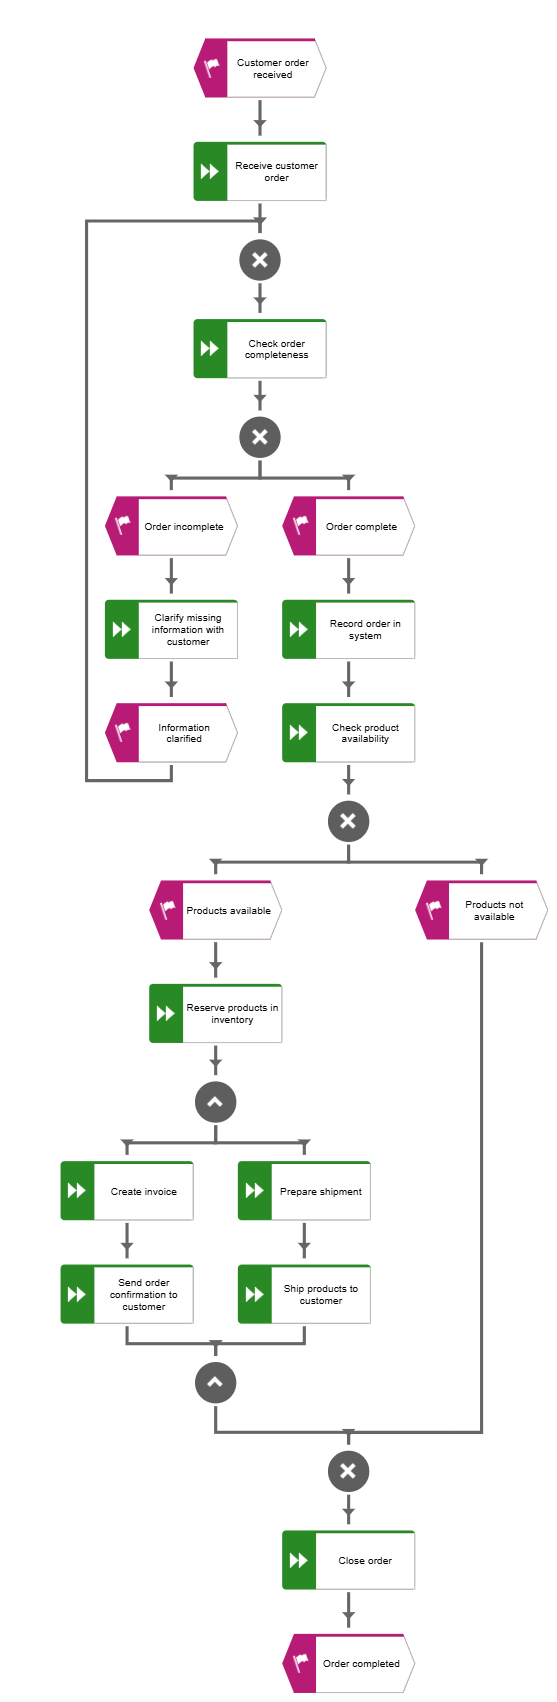
\includegraphics[width=0.4\textwidth]{Graphics/Test_EPC_Diagram.png}
    \caption{Beispiel eines modellierten Prozesses in EPK für eine Kundenbestellung}
    \label{fig:beispiel_epk}
\end{figure}

Ereignisse beschreiben Zustände eines Prozesses (bspw. ``Bestellung erhalten'' oder ``Produkt nicht verfügbar''), welcher den Verlauf eines Prozesses beeinflusst.\cite{gadatsch_grundkurs_2008}
Vergleichbar sind Ereignisse mit logischen Aussagen, dessen Ergebnisse wahr oder falsch sind. Somit kann man diese als boole'schen Aussagen interpretieren. Funktionen (oder auch Aktivitäten) hingegen beschreiben 
eine Tätigkeit oder eine Aufgabe eines Geschäftsprozesses (bspw. ``Prüfe den Produktbestand'' oder ``Erstelle Rechnung'') und überführen einen Eingangszustand in einen Ausgangszustand \cite{gadatsch_grundkurs_2008}. Dies kann man mit Anweisungen im Programmcode 
interpretieren. Funktionen können dabei Datenobjekte enthalten, um benötigte und resultierende Daten zu modellieren. Außerdem können organisatorische Einheiten und benötigte Software 
an eine Funktion gebunden werden. EPK ermöglicht es Funktionen in sich in Teilfunktionen aufzuteilen. Ist es nicht mehr möglich eine Funktion weiter aufzuteilen, so spricht man von einer Elementarfunktion. Ereignisse und Funktionen können durch Kanten 
verbunden und in eine logische Reihenfolge gebracht werden. Dadurch wird der
Ablauf eines Prozesses und auch der Datenfluss beschrieben. \cite{gadatsch_grundkurs_2008} 

Gemäß der EPK-Syntax gilt, dass ein Prozess mit einem Start-Ereignis beginnen und mit einem End-Ereignis enden muss. End-Ereignisse können dabei 
neue Prozesse auslösen. Auf ein Ereignis muss eine Funktion folgen \cite{gadatsch_grundkurs_2008}, jedoch können auf Funktionen weitere Funktionen folgen oder Ereignisse. Um auf der 
Basis einer Funktionsausgabe Entscheidungen zu treffen, gibt es Verknüpfungsoperatoren, welche es ermöglichen die Ausgabe einer Funktion mit den benachbarten
Ereignissen abzugleichen und einem Entscheidungsweg im Prozess zu folgen.\cite{gadatsch_grundkurs_2008} Ein Beispiel wäre die Überprüfung der Kreditwürdigkeit eines Kunden als Funktion. Je nachdem
welches Ereignis (bspw. ``Kreditwürdig'' oder ``Nicht kreditwürdig'') gemäß der Verknüpfung zutrifft, wird der entsprechende Entscheidungsweg genommen. 

TODO: Verknüpfungsoperatoren definieren mit Rump und Gadatsch als Quelle

In dieser Arbeit wird eine reduzierte Fassung von EPK betrachtet, welche azyklisch ist, das Datenobjekt nicht enthält und Funktionen elementar sind.

\subsection{Geschäftsprozessorchestrierung}

Unter Geschäftsprozessorchestrierung versteht man die Ausführung und Verwaltung von Geschäftsprozessen. \cite{kampik_agent-based_2019}

Seidlmeier definiert die Steuerung eines Prozesses von einer organisatorischen Einheit als Orchestrierung. \cite{seidlmeier_prozessmodellierung_2019}

In dieser Arbeit wird Geschäftsprozessorchestrierung umgesetzt durch Ausführung der Prozesschritte gemäß der Modellierung.

\section{Prozessautomatisierung}

Gemäß Heinrich und Lutz J. versteht man unter Automatisierung
den Vorgang [...] von Arbeitsgängen [...], die ohne unmittelbare menschliche 
Tätigkeiten ausgeführt werden. \cite{heinrich_wirtschaftsinformatik-lexikon_1989}

Dumas et. al definieren die Prozessautomatisierung als "die Konfiguration oder Implementierung eines IT-Systems [...], um den zukünftigen Prozess
zu unterstützen." \cite{dumas_grundlagen_2021}

\section{ARIS-Toolset}

Das ARIS-Toolset ist gemäß Scheer ein [...] Softwaresystem zur Analyse, Modellierung und
Navigation von Geschäftsprozessen. [...] Die Grundlage für das ARIS-Toolset wird von der 
Repository-Struktur gelegt, welche sich aus dem Konzept des ARIS-Haus gebildet hat. \cite{scheer_aris_1994}

Nach Leimeister ARIS bietet also eine Umsetzung prozessorientierter Organisationsgestaltung [...] an. Der Anspruch liegt dabei auf der 
Reduktion der Komplexität der Prozessmodellierung durch Spaltung der Unternehmensarchitektur durch die ARIS Methode in fünf 
Beschreibungssichten: \cite{leimeister_einfuhrung_2015}

\begin{itemize}
    \item Organisationssicht (``[...]Organisationseinheiten der Aufbauorganisation des Unternehmens'')\cite{leimeister_einfuhrung_2015}
    \item Funktionssicht (``Betriebswirtschaftlich relevante Funktionen[...]'')\cite{leimeister_einfuhrung_2015}
    \item Datensicht (``[...]Betriebswirtschaftlich relevante Funktionsobjekte[...]'')\cite{leimeister_einfuhrung_2015}
    \item Leistungssicht (``[...] Sach- oder Dienstleistungen als Ergebnisse von Prozessen[...]'')\cite{leimeister_einfuhrung_2015}
    \item Steuerungs-/und Prozesssicht (``[...] Zusammenhänge der zuvor genannten Beschreibungssichten in zeitlich-sachlogischen Beziehungen [...]'') \cite{leimeister_einfuhrung_2015}
\end{itemize}

Seidlmeier wiederum definiert ARIS als Produktgruppe, welche auf die Optimierung von Unternehmensprozessen zielt. Einige der Produkte in der Gruppe: \cite{seidlmeier_prozessmodellierung_2019}

\begin{itemize}
    \item ARIS Business Strategy
    \item ARIS Architect
    \item ARIS Cloud
    \item ARIS Simulation
    \item ARIS Process Governance 
    \item ARIS Process Mining
\end{itemize} \cite{seidlmeier_prozessmodellierung_2019} \cite{software_gmbh_aris_nodate}

In dieser Arbeit werden die Produkte ARIS Business Architect und ARIS Simulation zur Implementierung des Prototypen verwendet.

\section{Eingebettete Systeme}

Nach Hünning und Thaller ist ein eingebettetes System "[...] ein durch Software kontrollierter Computer oder 
Mikroprozessor, der Teil eines größeren Systems ist, dessen primäre Funktion nicht rechenorientiert ist." \cite{huning_eingebettete_2019} \cite{thaller_software-engineering_1997}

Barr und Massa definierren ein eingebettetes System als eine Kombination aus Computer Hardware und Software mit zusätzlichen mechanischen und elektronischen Bauteilen, 
um eine spezifische Funktion zu erfüllen. [...] Der Kontrast dazu ist der PC, bei welchem der Hersteller nicht weiß, wofür dieser verwendet wird. [...] ``Eingebettete 
Systeme sind oft eine Komponente in einem größeren System. Beispielsweise enthalten moderne Autos und LKW's viele eingebettete Systeme. Ein eingebettetes System ist 
für das ABS zuständig, ein anderes überwacht und steuert die Emissionen des Fahrzeugs, während ein drittes die Informationen dem Nutzer am Cockpit anzeigt.'' \cite{barr_programming_2006}

Prozessoren, welche dabei in eingebetteten Systemen verwendet werden sind Mikroprozessoren, Mikrocontroller und DSP-Chips.\cite{barr_programming_2006} \cite{marwedel_eingebettete_2008} In dieser Arbeit wird ein Mikrocontroller des
Herstellers Espressif Systems (Shanghai, China) verwendet.

\subsection{ESP32}

Der ESP32 ist ein Mikrocontroller \cite{hercog_design_2023} des Herstellers Esperssif Systems (Shanghai, China) und bietet einen Zweikern-Prozessor, integrierte WLAN und Bluetooth
Anbindung, GPIO Pins und hat einen niedrigen Stromverbrauch, weshalb dieser sehr oft für IoT-Anwendungen genutzt wird. \cite{hercog_design_2023} \cite{farhan_real-time_2026}
Neben den angegebenen Features, verfügt der ESP32 über Peripherien wie SPI, I2C, I2S, CAN, UART, etc. \cite{brandes_mikrocontroller_2024} Folgende Modelle werden dabei von Espressif Systems angeboten:

\begin{itemize}
    \item ESP32-WROOM-32
    \item ESP32-WROOM-32D
    \item ESP32-WROOM-32U
    \item ESP32-SOLO-1
    \item ESP32-WROVER (PCB)
    \item ESP32-WROVER (IPEX)
    \item ESP32-WROVER-B
    \item ESP32-WROVER-IB
\end{itemize} \cite{brandes_mikrocontroller_2024}

Den ESP32 kann man mit verschiedenen Programmiersprachen und Werkzeugen programmieren. In dieser Arbeit wird die ESP-IDF (Espressif IoT Development Framework) des Herstellers verwendet, 
welche Bibliotheken und Werkzeuge für die Entwicklung des ESP32 bietet. \cite{hercog_design_2023}

\section{IoT}

Es gibt keine eingdeutige Definition für IoT. Das Internet Architecture Board definiert es beispielsweise [...] als eine Menge an zahlreichen
eingebetteten Geräten, welche Kommunikationsdienste auf der Basis von Internetprotokollen anbieten. Diese Geräte werden gänig als \"Objekte"
oder \"Smarte Objekte" bezeichnet. Diese Objekte kommunizieren miteinander und brauchen keinen menschlichen Einfluss. \cite{balas_internet_2019}\cite{tschofenig_architectural_2015}\cite{wendzel_it-sicherheit_2018}

\subsection{CoAP}

Gemäß RFC7252 ist CoAP [...] ein spezialisiertes Internettransferprotokoll, welches für eingeschränkte Knoten und Netzwerke genutzt wird.
Diese Knoten haben meißt einen 8-Bit Mikrocontroller mit kleinen ROM und RAM. Eingeschränkte Netzwerke sind beispielsweise IPv6 über Low-Power WPAN,
welche eine hohe Paketfehöerrate und einen typischen Durchfluss von 10s bei kbit/s hat. Das Protokoll ist konzipiert für Maschine zu Maschine Anwendungen wie etwa
Smart-Energie oder Bauautomatisierung. \cite{thaller_software-engineering_1997}\cite{wendzel_it-sicherheit_2018}
CoAP baut dabei auf UDP auf und bringt damit einen komapkten Header mit. Zudem können CoAP-Clients auch Dienste und Resourcen selbst finden. \cite{wendzel_it-sicherheit_2018}
Dies wird in RFC7252 auch Resource Discovery genannt und geschieht über das Constrained RESTful Environments Link Format, was in RFC6690 beschrieben wird. \cite{shelby_constrained_2014}

Die direkte Suche von Resourcen ist meist nicht effizient oder praktikabel, da Geräte nicht ansprechbar sind oder sich in Netzwerken befinden, wo Multicast nicht effizient ist. Um die Suche also 
efiizienter zu gestalten gibt es sogenannte Resource Directorires, welche Buch führen über Resourcen auf anderen Servern. Das Format, was dabei genutzt wird entspricht auch RFC6690. \cite{amsuss_constrained_2022}

\subsection{MQTT}

Wendzel definiert MQTT als ein Protokoll, was auch in resourcenbeschränkten Situationen eingesetzt werden kann. Im Vergleich zu CoAP jedoch, verwendet MQTT eine Publish Subscribe Architektur, wodurch
Daten nicht abgefragt werden. Stattdessen wird man über Veränderungen von Werten informiert. \cite{wendzel_it-sicherheit_2018} Geräte, die die Daten zur Verfügung stellen werden dabei als Publisher bezeichnet, während Empfänger dieser 
Daten als Subscriber definiert werden. Verteilt werden die Daten an die Subscriber über einen Broker: einem Verteiler, wo Publisher Daten teilen und von Subscribern angenommen werden. Hierbei haben Publisher und
Subscriber keine Kenntnis voneinander. \cite{wendzel_it-sicherheit_2018} \cite{hunkeler_mqtt-s_2008}

\section{Sockets}

Unter einem Socket versteht man eine "Verallgemeinerung des Mechanismus für den Dateizugriff unter UNIX, das einen Endpunkt für die Kommunikation bereitstellt.
[...] Der wesentliche Unterschied zwischen Datei- und Socket-Deskriptioren besteht darin, dass das Betriebssystem einen Datei-Deskriptor an eine bestimmte Datei
oder ein bestimmtes Gerät bindet,[...], aber es kann Sockets erstellen, ohne sie an bestimmte Zieladressen binden zu müssen. Die Applikation kann jedes Mal, wenn sie das 
Socket nutzt [...], eine Zieladresse angeben[...] (z.B. wenn eine TCP-Verbindung aufgebaut wird)"\cite{comer_tcpip_2003} Nach Inden bieten Sockets dabei eine streambasierte 
Kommunikationsmöglichkeit, um Daten bidirektional zu übertragen. \cite{inden_weg_2020}

\section{WebSockets}

Gemäß RFC6455 versteht man unter WebSockets ein Kommunikationsprotokoll, das Browser basierten Anwendungen
eine bidirektionale Verbindung zum Server ermöglicht. Diese wurden davor mit mehreren HTTP-Anfragen realisiert, 
während WebSockets mittels eines Handshakes via HTTP, eine WebSocket Verbindung anfragt und man nach erfolgreichem 
Handshake eine bidirektionale Verbindung aufgebaut hat. \cite{fette_websocket_2011}